% ============================================================
% 片段：s03a  对应原文 section2.tex 第 647--877 行；PDF 第 24--32 页
% 内容：§3 Anomalies and SPT（3.1 及其三个小节）
% 译者：t-s03a   审校状态：初稿
% ============================================================

% ==== 原文 PDF 第 24 页 ====
\section{反常与 SPT}\label{sec:anomalies}

\begin{keytakeaways}
  \begin{itemize}[leftmargin=1.4em,itemsep=2pt,topsep=2pt]
    \item \textbf{物理图像}：'t Hooft 反常用整体对称性与规范不变性的冲突来刻画——把整体对称性推广为背景规范场后，配分函数在局域规范变换下不再不变，而是多出一个相位因子。该相位无法靠局域抵消项消去，只能由高一维的 SPT 体通过反常流入（anomaly inflow）吸收。
    \item \textbf{数学工具}：群上同调。0+1 维反常与 1+1 维 SPT 由 $H^2_{\rm grp}(G,U(1))$ 分类；1+1 维反常与 2+1 维 SPT 由 $H^3_{\rm grp}(G,U(1))$ 分类。上闭链条件正是结合律（0+1 维）与五边形方程（1+1 维）的体现，上边缘则对应可自由重定义的局域抵消项。
    \item \textbf{关键结论}：SPT 相的边界必然带有非平凡 't Hooft 反常，因此非平凡 SPT 相不可能拥有既保持能隙、又保持对称性、且不含拓扑序的边界。
    \item \textbf{关键例子}：Haldane 链是受 $SO(3)$（或其子群 $\mathbb{Z}_2\times\mathbb{Z}_2$）保护的 SPT 相，其边界自旋-$\frac{1}{2}$ 构成 $SO(3)$ 的投影表示，对应第二 Stiefel--Whitney 类 $\frac{1}{2}w_2$；AKLT 模型的四重简并基态给出该边界自由度的显式实现。
  \end{itemize}
\end{keytakeaways}

本节将在前文关于对称性的综合视角下回顾 't Hooft 反常（'t Hooft anomaly），并说明其与 SPT 相（symmetry-protected topological phase，对称保护拓扑相）的联系~\cite{chen2011two,chen2012chiral,elsenayak2014,kapustin2014anomalous,kapustin2014anomalies,kapustin2014symmetry,thorngren2015higher,wang2015bosonic,chenjie2016,bultinck2018global,wan2018higher,wang2018symmetric,TI4,TI5}。第~\ref{sec:anomaly-SPT}~节的讨论集中于 't Hooft 反常与高一维 SPT 相之间的关系；为简单起见，重点放在 1 维与 2 维的反常上，并以凝聚态物理中一个众所周知的例子来说明：Haldane 链边界上带反常的自旋-$\frac{1}{2}$。第~\ref{sec:gen-SPT}~节面向进阶读者，深入探讨 't Hooft 反常与 SPT 相的一般分类，涉及高维系统、高形式对称性、费米子系统与配边等较复杂的主题。该部分虽有价值，但超出入门水平，初学者可以先行跳过、日后再读。

\subsection{SPT 边界上的 't Hooft 反常}\label{sec:anomaly-SPT}

对于由作用量 $S[\phi]$ 描述、含物质场 $\phi$ 的理论，首先必须明确\emph{整体}对称性的含义：它可以是离散的，未必由无穷小变换生成。我们先指定物质场的对称变换，对每个 $g\in G$ 记 $\phi\mapsto \phi^g$，其中 $G$ 表示对称群。物质场 $\phi$ 的量子系统要具有整体对称群 $G$，要求在这些变换下满足
\begin{align}\label{gaugetransf}
S[\phi] = S[\phi^g] \quad \text{且} \quad \mathcal{D}\phi = \mathcal{D}\phi^g, \quad \forall g\in G.
\end{align}
此时称由配分函数 $Z = \int \mathcal{D}\phi \exp(iS[\phi])$ 定义的理论具有由群 $G$ 刻画的整体对称性。

下面把背景规范场（background gauge field）$A$ 耦合到理论中，考察其推论。这里所谓背景规范场，是指只对物质场 $\phi$ 作积分，而把规范场 $A$ 固定：
\be Z[A] = \int\mathcal{D}\phi e^{iS[A,\phi]} \ . \ee

% ==== 原文 PDF 第 25 页 ====
当 $Z[A]$ 不等于 $Z[A^g]$、即 $Z[A]$ 在\emph{局域}规范变换下不再保持不变时，就出现 't Hooft 反常。的确，由于 $Z[A]$ 不具备规范不变性，对规范场 $A$ 作积分（integrate out）便成为问题：我们实际上是在规范场 $A$ 的规范轨道上积分。为处理这一点，引入 $Z[A]$ 中对 $A$ 作规范化（gauging）存在障碍这一概念，该障碍由下式描述：
\be
Z[A^g] = Z[A]\cdot Z_{\text{anomaly}} [A,g],
\ee
其中 $g$ 表示\emph{局域}规范变换，而不是式~(\ref{gaugetransf}) 中的整体变换。相位因子 $Z_{\text{anomaly}}[A,g] \in U(1)$ 刻画该理论的 't Hooft 反常。

\begin{yizhu}
式 (3.3) 中的 $Z_{\text{anomaly}}[A,g]$ 不是 $A$ 与 $g$ 的任意相位：把两次局域变换复合为一次时，它必须满足上闭链型的相容条件，因此其取值是离散的，构成由 $H^{d+1}(BG,U(1))$ 刻画的离散数据（即反常系数）。这正解释了 't Hooft 反常为何不能靠加局域抵消项消除：抵消项只能改变上边缘，改变不了上同调类。另需注意 $Z[A]$ 只对物质场积分、$A$ 保持固定，故 $Z_{\text{anomaly}}$ 一般不是 $A$ 的局域泛函。
\end{yizhu}

从第~\ref{sec:three}~节所讨论的关于物理系统对称性的三个视角来看，'t Hooft 反常揭示如下含义：
\begin{enumerate}
\item \textbf{拓扑缺陷网络（TDN）视角}。在此视角下，$G$-对称性缺陷失去拓扑性质。特别地，当通过时空中拓扑缺陷的重新连接这类局域操作改变网络的拓扑时，会额外出现相位因子；这些额外相位因子正是对称性反常的标志。
\item \textbf{平坦联络视角}。这里，TDN 的局域变换可以翻译为规范场的规范变换。于是，配分函数在 TDN 局域改变下不再保持不变这一事实，就翻译为等价的规范场联络给出不同的配分函数，换言之 $Z[A^g]\neq Z[A]$。
\item \textbf{分类空间视角}。在此视角下，规范变换与映射 $\phi: M^d\rightarrow B^{p+1}G$ 的同伦性质相关。因此，带反常的配分函数 $Z: [M^d, B^{p+1}G]\rightarrow \mathbb{C}$ 并不是同伦类 $[\phi]$ 上的良定义函数（$[\phi]$ 表示 $M^d$ 到 $B^{p+1}G$ 的映射同伦类），而依赖于同伦类 $[\phi]$ 中映射 $\phi$ 的具体选取。
\end{enumerate}

\subsubsection{0+1 维 't Hooft 反常与 1+1 维 SPT}
\label{subsubsec:0+1D}

考虑一个具有 0-形式整体对称性 $G$ 的 0+1 维系统。在这个一维时空中，群元 $g\in G$ 的作用由插入一个作用在系统希尔伯特空间上的点算符 $U_g$ 来体现。由于整体对称性的性质，$U_g$ 插入的精确位置没有意义。再者，$U_h$ 与 $U_g$ 的相继作用完全等价于单个算符 $U_{gh}$ 的作用。这一等价关系可以理解为一次改变 TDN 拓扑的局域操作。
% ==== 原文 PDF 第 26 页 ====
数学上，这一关系写成
\be
U_gU_h=U_{gh}.
\ee
该式表明，$U_g$ 的作用在 0+1 维系统的希尔伯特空间上构成群 $G$ 的线性表示。

\begin{yizhu}[原文疑误]
源码与 PDF 中有三处小疵，均照原文保留：其一，第 25--26 页（印刷页码）出现“the topology of the topology of TDN”的重复，译文按本义只作一次拓扑理解；其二，第 28 页（印刷页码）对式 (3.11) 的引用写作 Eq.~(ref\{eq:tri\})，缺一个反斜杠，PDF 中实际排成 (refeq:tri)；其三，第 29 页（印刷页码）“This is believed to leads to a gapless state”中 leads 应为 lead。
\end{yizhu}

反之，若放松 TDN 在局域操作下保持不变这一假设，则引入修改后的方程
\be\label{UgUhUgh}
U_gU_h = \omega(g,h) U_{gh}.
\ee
这里 $\omega: G\times G \rightarrow U(1)$ 引入一个额外的相位因子。必须注意，这个相位因子 $\omega$ 并非任意：希尔伯特空间上的 $G$-作用必须满足结合律，由此得到要求
\be\ba
&\quad (U_g\cdot U_h)\cdot U_k = U_g\cdot (U_h\cdot U_k)\cr
&\Rightarrow \omega(g,h)\omega(gh,k) U_{ghk} = \omega(g,hk)\omega(h,k) U_{ghk}\cr
&\Rightarrow\omega(g,h)\omega(gh,k)  = \omega(g,hk)\omega(h,k). \cr
\ea\ee
这一相容性条件可以解释为群上同调中的 2-上闭链条件，确切地说：
\be (\dd_2 \omega) (g,h,k) := \frac{\omega(h,k)\omega(g,hk)}{\omega(gh,k)\omega(g,h)} = 1. \ee
关于群上同调的更完整讨论，参见附录~\ref{App:GrpChmlg}。

\begin{yizhu}
式 (3.7) 与 (3.10) 采用的是乘法记号的群上同调：$\dd_2$ 表达式中分子与分母的次序对应一种归一化约定；若把群运算写成加法（$G$ 阿贝尔、相位写成 $\mathrm{e}^{i\alpha}$），它等价于 $\dd\alpha=\alpha(h,k)-\alpha(g,hk)+\alpha(gh,k)-\alpha(g,h)$。推导 (3.6) 时隐含假设了 $U_{ghk}$ 可逆、可从两边消去；这对 $U(1)$ 相位因子自动成立，但对一般算符需另作说明。此外 (3.7) 写 $\dd_2$、(3.19) 写 $\dd$，二者分别是 2-上边缘与 3-上边缘算子，不要与 (3.9) 中的 $\dd_1$ 混为同一符号。
\end{yizhu}

通过引入相位因子 $\lambda(g)$，可以修改作用在系统希尔伯特空间上的对称性作用 $U_g$ 的定义：
\be
U_g \mapsto U_g' = \lambda(g) U_g.
\ee
这一修改的效果是把 2-上闭链 $\omega$ 变为新函数
\be
\omega(g,h)\mapsto \omega'(g,h )= \omega(g,h)\lambda(h)   \lambda(g)\lambda(gh)^{-1} =(\omega\cdot \dd_1\lambda)(g,h) \ . 
\ee
注意 ${\text{im}(\dd_1)}$ 中的元素可以解释为一个整体 $U(1)$ 相位，它只是描述量子系统时所作的一种选择，没有物理意义，因此在我们的描述中应当被商掉。于是相位因子 $\omega$ 是群 $G$ 的第二上同调群的元素，定义为：
\be H^2_{\rm grp}(G,U(1))  =  \frac{{\rm ker}(\dd_2)} {{\rm im}(\dd_1)} \ . \ee
指定一个相位因子 $\omega \in H^2_{\text{grp}}(G, U(1))$，等价于定义群 $G$ 的一个投影表示（projective representation）。

% ==== 原文 PDF 第 27 页 ====
以上分析揭示了 0+1 维量子场论中 't Hooft 反常与上同调群 $H^2_{\rm grp}(G,U(1))$ 之间的有趣联系。该上同调群是分类群 $G$ 的投影表示的关键工具。有趣的是，上同调群 $H^2_{\rm grp}(G,U(1))$ 在物理中还有另一项关键作用：它是 1+1 维 SPT 态的分类方案~\cite{SPT1D1,SPT1D2,SPT1D3,SPT1D4}。SPT 相是由对称性提供非平凡保护的有能隙物态。值得注意的是，以 $\omega \in H^2_{\rm grp}(G,U(1))$ 刻画 't Hooft 反常的 0+1 维量子场论，与同样带有该 $\omega$ 的 1+1 维 $G$-SPT 相之间存在直接对应。这一对应表明，带 't Hooft 反常的 0+1 维量子场论可以看作 1+1 维 SPT 相的边界理论。因此，非平凡 SPT 相不可能拥有既保持能隙、又保持对称性且不含拓扑序的边界，因为这样的边界必然带有非平凡 't Hooft 反常。

\begin{center}
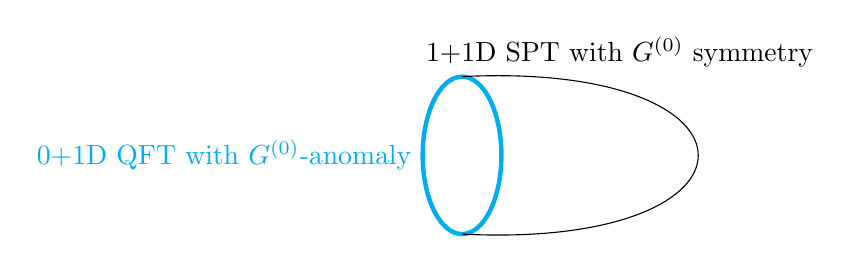
\begin{tikzpicture}
    \draw[ultra thick, cyan] (0,0) ellipse (0.5 and 1) (-0.5,0)node[left]{0+1D QFT with $G^{(0)}$-anomaly} ;
    \draw (0,1) .. controls (4,1.2) and (4,-1.2) .. (0,-1) (2,1)node[above]{1+1D SPT with $G^{(0)}$ symmetry};
\end{tikzpicture}
\end{center}

为理解 0+1 维 't Hooft 反常与 1+1 维 SPT 相之间的关系，可以从显式构造 1+1 维 SPT 系统在格点上的配分函数入手。定义该配分函数的步骤如下：
\begin{enumerate}
    \item 为 1+1 维闭时空流形 $M$ 选取一个三角剖分。
    \item 用 $G$ 中的群元标记三角剖分的每条边，并要求在每个三角形内满足平坦联络条件，即
    \be\label{eq:tri}
        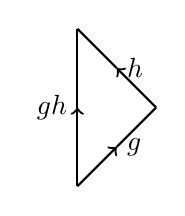
\begin{tikzpicture}
            \draw[thick,->] (0,0)--(0,1);
            \draw[thick] (0,1)--(0,2) (0,1)node[left]{$gh$};
            \draw[thick,->] (0,0)--(0.5,0.5)  node[right]{$g$};
            \draw[thick] (0.5,0.5)--(1,1);
            \draw[thick,->] (1,1)--(0.5,1.5) node[right]{$h$};
            \draw[thick] (0.5,1.5)--(0,2);
        \end{tikzpicture}
    \ee
    这种边标号本质上给出平坦联络 $A: M \to BG$ 的离散表示：$M$ 中每条不同路径对应一个群元，它由沿各条链路的群元相乘得到。
    \item 每个基本三角形（一般维数下为单纯形）为配分函数贡献一个元素 $\omega_2(g, h)^{\pm 1} \in U(1)$，符号 $\pm$ 随三角形的定向而变。
    % ==== 原文 PDF 第 28 页 ====
    函数 $\omega_2$ 可以解释为映射 $ BG \to B^2 U(1) $，由于同构
    \be [BG, B^2U(1)]\cong H^2(BG,U(1))\cong H_\mathrm{grp}^2(G,U(1)).  \ee
    它落在第二上同调群 $H^2(BG, U(1))$ 中。
    \item 对任意平坦联络构型 $A$，配分函数表示为 $\omega_2$ 在全部三角形上的乘积，并计入各三角形的定向~\cite{chen2013symmetry}：
    \be Z[A] =  \exp{i \int_M L} = \prod_{\Delta} e^{iL(\Delta)} = \prod_{\Delta} \omega_2 (A(\Delta)) = \prod_{\Delta}A^* (\omega_2)(\Delta).
    \ee
\end{enumerate}

\begin{yizhu}
式 (3.11) 的三角形把两条边标为 $g$ 与 $h$、第三条边标为 $gh$，这等价于要求沿这个闭三角形走一圈所得的群元之积为单位元，即联络平坦。注意其中隐含了定向约定：箭头指明行走方向，逆着箭头走时该边的标号取逆元 $g^{-1}$，而作者并未写出这一点；但判断 $\omega_2(g,h)$ 取 $+1$ 还是 $-1$ 恰恰需要它（这正是第 3 步中符号 $\pm$ 的来源）。在更一般维数下，同一条件表现为 $(p+1)$-单纯形各面上标号的相容性。
\end{yizhu}

这一构造给出了定义 1+1 维 SPT 系统配分函数的普适方式：它以三角剖分中的边标号为基础，并计入各个三角形的贡献，从而在配分函数与上同调类 $ \omega_2 \in H^2_\mathrm{grp}(G,U(1))$ 之间建立起直接对应。

当考察开的 1+1 维时空流形时，0+1 维 't Hooft 反常与 1+1 维 SPT 相之间的复杂关系变得格外透明。具体地，考虑边界附近的一个三角形，如式~(ref{eq:tri}) 所示。去掉这样一个三角形可以理解为一次边界局域操作，它使边界边的数目改变一条。在此语境下，边上的每个群元标号对应对偶 TDN 表示中算符 $U_g$ 的插入。当边界附近的一个三角形被去掉时，边界上的对称性作用从 $U_{gh}$ 变为 $U_gU_h$。这一改变导致相位出现偏差，即式~(\ref{UgUhUgh}) 中的 $\omega(g,h)$，它正是 't Hooft 反常的标志。值得注意的是，该相位因子恰好抵消被去掉的三角形对 1+1 维体 SPT 配分函数的贡献。这揭示了一般的反常流入（anomaly inflow）机制：包含边界与体的组合系统仍保持物理自洽性与规范不变性。这一认识确认，非平凡 SPT 态不可能具有平凡有能隙的对称边界，因为边界理论表现出非平凡 't Hooft 反常。

\subsubsection{例：Haldane 链边界上的反常自旋-$1/2$}

为深入考察体--边对应这一现象，来看一个奠基性的例子：1+1 维 Haldane 链~\cite{haldane1983nonlinear,haldane1983continuum} 与其带反常的 0+1 维自旋-$\frac{1}{2}$ 边界之间的关系。该例说明 't Hooft 反常如何与高一维的 SPT 相联系。

Haldane 链是 1+1 维自旋-$s$ 链，其海森堡相互作用为
\be\label{eq:Haldane}  H = \sum_{\expval{ij}} \vb{S}_i\cdot \vb{S}_j. \ee
% ==== 原文 PDF 第 29 页 ====
在低能极限下，Haldane 证明该模型可被一个连续量子场论有效描述，其配分函数为
\be\ba 
Z &= \int \mc{D} \vb{n} \exp(i\int_{M^2} (\ptl_\mu \vb{n} )^2 \dd^2 x + i  \theta \mathcal{N}[\vb{n}]  ),
\ea\ee
其中 $\mathcal{N}$ 表示场 $\mathbf{n}: M^2 \rightarrow S^2$ 的绕数（即映射度）。第二项中的参数 $\theta=2\pi s$ 与链的自旋 $s$ 有关。

对整数自旋 $s$，由于 $\mathcal{N}$ 取整数，第二项 $e^{i\theta \mathcal N}$ 在闭流形 $M^2$ 上积分后化为 $e^{2\pi i} = 1$。因此，若只保留第一项非线性 sigma 模型，理论在重整化群流下将流向有能隙的对称无序态。相反，对半奇数自旋 $s$，该项依 $\mathcal{N}$ 的奇偶取 $\pm 1$，从而在路径积分中导致相消干涉，据信这给出无能隙态。对反铁磁 1+1 维海森堡模型，$s$ 的这种有能隙/无能隙依赖关系称为 Haldane 猜想~\cite{haldane1983nonlinear,haldane1983continuum}。

自旋-1 Haldane 链的非平凡边缘态可以通过开 1+1 维链的配分函数来理解。沿 0+1 维边界，$\theta$ 项变为自旋-$1/2$ 系统的 Wess--Zumino--Witten 模型~\cite{ng1994edge}。1+1 维体中的自旋-1 自由度（d.o.f.）与边界上的自旋-$1/2$ 自由度之间的关键差别在于其对称群：自旋-1 自由度构成自旋转动对称群 $SO(3)$ 的线性表示，而自旋-$1/2$ 自由度构成 $SU(2)$ 的线性表示、同时构成 $SO(3)$ 的投影表示。由此可以看出，Haldane 链是受 $SO(3)$ 自旋转动对称性保护的 SPT 态~\cite{gu2009tensor}。其边界对应一个自旋-$1/2$ 系统，具有分数化荷，无法在保持对称性的前提下被打开能隙。因此，0+1 维自旋-$1/2$ 的 $SO(3)$ 't Hooft 反常被受同一 $SO(3)$ 群保护的 1+1 维 SPT 体抵消。边界 't Hooft 反常与体内 SPT 相之间的这一有趣关系，阐明了对称性与拓扑在 Haldane 链独特性质中的作用。

要更直接地看出自旋-1 Haldane 链的边界是具有 $SO(3)$ 投影表示的自旋-$1/2$，可以借助 AKLT 模型~\cite{affleck2004rigorous}。该模型可图示如下：
\begin{center}
    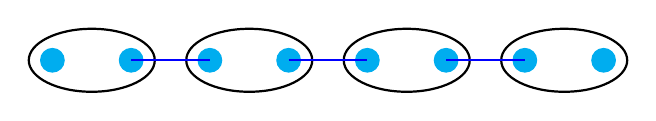
\begin{tikzpicture}
        \filldraw[cyan] (0,0) circle (0.15);
        \filldraw[shift = {(1,0)},cyan] (0,0) circle (0.15);
        \filldraw[shift = {(2,0)},cyan] (0,0) circle (0.15);
        \filldraw[shift = {(3,0)},cyan] (0,0) circle (0.15);
        \filldraw[shift = {(4,0)},cyan] (0,0) circle (0.15);
        \filldraw[shift = {(5,0)},cyan] (0,0) circle (0.15);
        \filldraw[shift = {(6,0)},cyan] (0,0) circle (0.15);
        \filldraw[shift = {(7,0)},cyan] (0,0) circle (0.15);
        \draw[thick] (0.5,0) ellipse (0.8 and 0.4 );
        \draw[shift = {(2,0)}, thick] (0.5,0) ellipse (0.8 and 0.4 );
        \draw[shift = {(4,0)}, thick] (0.5,0) ellipse (0.8 and 0.4 );
        \draw[shift = {(6,0)}, thick] (0.5,0) ellipse (0.8 and 0.4 );
        \draw[thick,blue] (1,0)--(2,0);
        \draw[shift = {(2,0)},thick,blue] (1,0)--(2,0);
        \draw[shift = {(4,0)},thick,blue] (1,0)--(2,0);
        
    \end{tikzpicture}
\end{center}
这里，蓝点代表自旋-$1/2$ 粒子；包围两个自旋-$1/2$ 粒子的椭圆表示投影到每个格点上的自旋-1 三重态；连接两个自旋-$1/2$ 粒子的蓝线表示二者之间的单态。
% ==== 原文 PDF 第 30 页 ====
可以证明，哈密顿量~\cite{affleck2004rigorous}
\be
H_\mathrm{AKLT} = \sum_{\expval{ij}} \left[ \vb{S}_i\cdot \vb{S}_j + \frac{1}{3} (\vb{S}_i\cdot \vb{S}_j)^2 \right]
\ee
的基态恰为上图所示的态。数值计算确认，AKLT 模型与式~(\ref{eq:Haldane}) 中的反铁磁海森堡模型属于同一相，其间没有相变。在闭合的一维空间环上，AKLT 模型的基态唯一；而在开链上，由于链两端存在悬垂的自旋-$1/2$ 粒子，基态为四重简并。因此可以显式看到，自旋-1 Haldane 链的边界是自旋-$1/2$ 系统，其 $SO(3)$ 对称性反常表现为投影表示而非线性表示。

\begin{yizhu}
开链基态是四重简并而非二重，可由边界条件的图像理解：开链两端各留一个悬垂的自旋-$\frac{1}{2}$（每个格点的自旋-1 由两个自旋-$\frac{1}{2}$ 投影得到，链端只余其中一个），每个悬垂自由度给出二重简并，两端相互独立，故简并度为 $2\times 2=4$。这也是 AKLT 模型对 SPT 相的存在性证明：它给出严格可解的基态，说明 Haldane 相与反铁磁海森堡模型同相（Haldane 猜想），而不必依赖数值结果；作者此处只提数值计算，未展开这一论证。
\end{yizhu}

从 SPT 相的角度看，1+1 维 Haldane 相受对称群 $SO(3)$ 或其子群 $\mathbb{Z}_2 \times \mathbb{Z}_2$ 保护。1+1 维 SPT 相与 0+1 维 't Hooft 反常都可以用对称群的投影表示来分类。具体地，可以考察 $SO(3)$ 与 $\mathbb{Z}_2 \times \mathbb{Z}_2$ 以 $U(1)$ 为系数的第二群上同调：
\be  H_\mathrm{grp}^2 (SO(3),U(1)) = H^2_\mathrm{grp} (\mathbb Z_2\times\mathbb Z_2,U(1)) = \bbZ_2. \ee
$H_{\text{grp}}^2 (SO(3),U(1)) = H^2(BSO(3),U(1)) $ 中的非平凡元素是第二 Stiefel--Whitney 类 $\frac{1}{2}w_2$。因此，1+1 维 $SO(3)$-SPT 的作用量为
\be
S=\frac{1}{2}\int \dd^2 x\ w_2.
\ee

\begin{yizhu}
式 (3.17)、(3.18) 把 $\frac{1}{2}w_2$ 当作 $H^2(BSO(3),U(1))=\mathbb{Z}_2$ 的非平凡元素，有两件事需要留意。其一，$w_2$ 本是取值于 $\mathbb{Z}_2$ 的第二 Stiefel--Whitney 类，它在 $H^2(\,\cdot\,,U(1))$ 中的像由 $\mathbb{Z}_2\subset U(1)$ 给出；写 $\frac{1}{2}w_2$ 时应把它理解为 $\theta=\pi$ 的拓扑项 $S=\frac{\theta}{2\pi}\int w_2$，于是 $S$ 只在模 $2\pi$ 的意义下确定，$\mathrm{e}^{iS}$ 只取 $\pm 1$。其二，若把 $w_2$ 取为整系数上链的具体代表，则改变代表只让 $S$ 改变 $2\pi$ 的整数倍，这正是该反常与 SPT 作用量良定义所要求的。
\end{yizhu}

此外，边界上出现自旋-$\frac{1}{2}$，也恰好对应 $SO(3)$ 或 $\mathbb{Z}_2 \times \mathbb{Z}_2$ 的非平凡投影表示；其 't Hooft 反常同样由第二 Stiefel--Whitney 类刻画。

这个例子清楚地展示了体--边对应（bulk-boundary correspondence）：位于边界上、带 't Hooft 反常的量子场论，恰好对应相应 SPT 态的边界。

\subsubsection{例：1+1 维反常与 2+1 维 SPT}

现在把时空维数提高一维：1+1 维中 $G$ 联络的局域操作对应二维 Pachner 移动，该移动引入一个依赖三个群元的相位因子 $\omega_3$：
% ==== 原文 PDF 第 31 页 ====
\begin{center}
    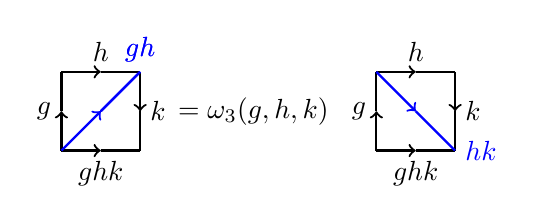
\begin{tikzpicture}
        \draw[thick , ->] (0,0) -- (0.5,0) node[below] {$ghk$};
        \draw[shift={(4,0)}, thick , ->] (0,0) -- (0.5,0) node[below] {$ghk$};
        \draw[thick ] (0.5,0) -- (1,0);
        \draw[shift={(4,0)}, ,thick ] (0.5,0) -- (1,0);
        \draw[thick,->] (0,0)--(0,0.5) node[left]{$g$};
        \draw[shift={(4,0)},thick,->] (0,0)--(0,0.5) node[left]{$g$};
        \draw[thick ] (0,0.5) -- (0,1);
        \draw[shift={(4,0)},thick ] (0,0.5) -- (0,1);
        \draw[thick, ->] (0,1) -- (0.5,1) node[above] {$h$};
        \draw[shift={(4,0)},thick, ->] (0,1) -- (0.5,1) node[above] {$h$};
        \draw[thick] (0.5,1)--(1,1) ;
        \draw[shift={(4,0)},thick] (0.5,1)--(1,1) ;
        \draw[thick , ->] (1,1)--(1,0.5) node[right]{$k$} node[right]{$\  \ \ = \omega_3(g,h,k)$};
        \draw[shift={(4,0)},thick , ->] (1,1)--(1,0.5) node[right]{$k$};
        \draw[thick] (1,0.5)--(1,0);
        \draw[thick,shift={(4,0)}] (1,0.5)--(1,0);
        
        \draw[thick, ->, blue] (0,0)--(0.5,0.5);
        \draw[thick, blue] (0.5,0.5)--(1,1) node[above]{$gh$};
        \draw[shift={(4,0)},thick,-> ,blue] (0,1)--(0.5,0.5);
        \draw[thick, blue] (0.5,0.5)--(1,1) node[above]{$gh$};
        \draw[shift={(4,0)},thick,blue] (0.5,0.5)--(1,0) node[right]{$hk$} ;
    \end{tikzpicture}.
\end{center}
从 2+1 维 SPT 体的角度看，相位因子 $\omega_3(g,h,k)$ 被赋给平坦联络 $A: M^3 \to BG$ 的一个四面体，即
\begin{center}
    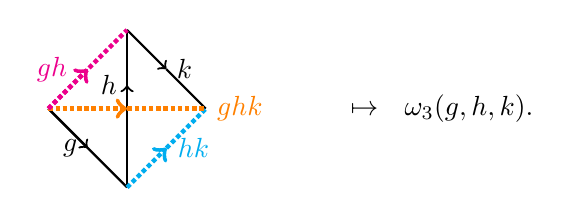
\begin{tikzpicture}
        \draw[->,thick] (0,0)--(0.5,-0.5) node[left]{$g$} ;
        \draw[thick] (0,0)--(1,-1)  ;
        \draw[->,thick] (1,-1)--(1,0.3) node[left]{$h$} ;
        \draw[thick] (1,0)--(1,1) ;
        \draw[->, thick] (1,1)--(1.5,0.5) node[right]{$k$};
        \draw[thick] (1.5,0.5)--(2,0) ;
        \draw[->, ultra thick,cyan,densely dotted] (1,-1)--(1.5,-0.5) node[right]{$hk$} ;
        \draw[ultra thick,cyan, densely dotted] (1.5,-0.5)--(2,0);
        \draw[ultra thick, orange,densely dotted] (0,0)--(2,0) node[right]{$ghk$};
        \draw[ultra thick, orange,densely dotted,->] (0,0)--(1,0);
        \draw[ultra thick, magenta,densely dotted,->] (0,0)--(0.5,0.5) node[left]{$gh \ $};
        \draw[ultra thick, magenta,densely dotted] (0,0)--(1,1);
        \node (a) at (5,0) {$ \mapsto  \ \ \omega_3(g,h,k)$.};
    \end{tikzpicture}
\end{center}
这里，$M^3$ 表示三维时空流形，$BG$ 表示对称群 $G$ 的分类空间（classifying space）。2+1 维 SPT 态的配分函数可表示为时空中各四面体所带相位因子的乘积。把所有这些相位因子的贡献计入后可以看到，原本存在于 1+1 维理论中的 't Hooft 反常被 2+1 维体 SPT 的影响所抵消。这一抵消机制保证了组合系统在对称性与拓扑性质两方面的自洽性。

存在一个支配相位因子 $\omega_3$ 的相容性条件。正如 0+1 维反常中 $\omega_2$ 必须是 2-上闭链，相位因子 $\omega_3$ 也必须满足类似要求，这可由下面的交换图直观表示：
\begin{center}
\begin{tikzcd}
&  & (g(hk))l \arrow[rr, "{\omega_3(g,hk,l)}"] & & g((hk)l) \arrow[rrd, "{\omega_3(h,k,l)}"] &  & \\
((gh)k)l \arrow[rrrd, "{\omega_3(gh,k,l)}"] \arrow[rru, "{\omega_3(g,h,k)}"] &  & & &   &  & g(h(kl)) \\
&  & & (gh)(kl) \arrow[rrru, "{\omega_3(g,h,kl)}"] & &  &         
\end{tikzcd}
\end{center}
上述条件正是 $\omega_3$ 的 3-上闭链条件：
\be
(\dd \omega_3)(g,h,k,l) = \frac{\omega_3(h,k,l) \omega_3(g,hk,l) \omega_3(g,h,k)}{\omega_3(gh,k,l) \omega_3(g,h,kl)} = 1.
\ee
3-上闭链条件作为五边形方程（pentagon equation）的特例，是保证相位因子 $\omega_3$ 在不同四面体之间相容、自洽的基本要求。满足该条件后，相位因子确保 SPT 态良定义且拓扑不变。这一条件对于确立 SPT 相的稳健性与稳定性至关重要，因为它保证系统的物理性质与对称性在各种三角剖分或时空分割下都保持不变。

% ==== 原文 PDF 第 32 页 ====
与 0+1 维反常、1+1 维 SPT 的情形类似，2+1 维 SPT 与 1+1 维反常的上闭链 $\omega_3$ 也存在“规范变换”。该变换来自用局域抵消项（counterterm）重新定义对称性作用。这些抵消项引入一个称为 3-上边缘（3-coboundary）的子群，在反常与 SPT 相的分类中必须把它商掉。因此，分类由第三上同调群 $H_{\mathrm{grp}}^3(G,U(1))$ 决定~\cite{chen2012symmetry,chen2013symmetry}。
